\subsubsection{Online-Speicher mit Wuala}
Wuala ist ein Cloud-Speicher der 5 GB Speicherplatz kostenlos anbietet, f�r mehr muss man bezahlen. Bezahlung f�r zus�tzlichen Speicher ist nur via PayPal.com auf der Webseite \href{https://www.wuala.com}{https://www.wuala.com} m�glich.\\

Man kann den Datenspeicher als Backup-Medium nutzen, Daten auf mehreren Rechnern synchronisieren oder im Team verteilen. Die Client Software verschl�sselt die Daten auf dem eigenen Rechner bevor sie in den Online-Speicher �bertragen werden. Die Software gibt es f�r Windows, Linux und MacOS sowie f�r Android ind iPhone.\\

Die \textbf{Installation} ist einfach.
\begin{itemize}
 \item F�r Windows steht auf der Webseite ein Setup-Programm zum Downlaod bereit. Nach dem Download ist das Programm zu starten und den Anweisungen des Assistenten zu folgen.
 \item F�r viele Linux-Derivate stehen Pakete auf der Downloadseite bereit. Vor der Installation sollte man zuerst die ben�tigte Java Runtime installieren und FUSE.
 \begin{verbatim}
  > sudo aptitude install default-jre fuse 
 \end{verbatim} 
 Alle Nutzer, die Wuala nutzen wollen, m�ssen zur Gruppe \textit{fuse} geh�ren:
 \begin{verbatim}
  > sudo addgroup USERNAME fuse
 \end{verbatim} 
 Danach kann man das Wuala-Paket installieren, f�r Debian und Ubuntu mit: 
\begin{verbatim}
 > sudo dpkg -i wuala*.deb
\end{verbatim} 
\end{itemize}

Beim ersten Start muss man einen Account anlegen. Das Passwort ist sehr wichtig! Es gibt keine M�glichkeit, an die Daten im Online-Speicher zu kommen, wenn man das Passwort vergessen hat. Es gibt auch keine M�glichkeit zum Passwort-Reset!  Die E-Mail Adresse ist unwichtig, es gibt nur eine Verwendung. Wenn man das Passwort vergessen hat, wird die Passwort-Merkhilfe an diese E-Mail Adresse gesendet. Wegwerf-Adressen werden akzeptiert.\\

\begin{figure}[htb]
\begin{center}
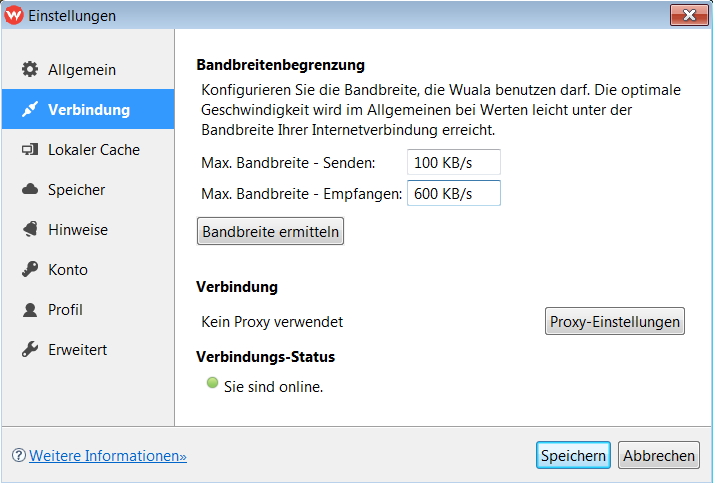
\includegraphics[scale=0.45]{../screenshots/wuala-config.png}
\caption{Wuala Konfiguration}
\label{abb:wualaconfig}
\end{center}
\end{figure}

In der Konfiguration kann man die Up- und Download Geschwindigkeit an den eigenen Internetzugang anpassen.\\

Mit einem HTTP-Proxy kann man die Verbindung zum Cloud-Speicher anonymisieren. JonDonym kann out-of-the-box als Anonymisierungsdienst verwendet werden. Bei der Nutzung von Premium-Diensten gibt es kaum Geschwindigkeitseinbu�en. Tor bietet nur einen SOCKS Proxy und kann deshalb nicht direkt verwendet werden. Man ben�tigt zus�tzlich eine HTTP-Proxy (Polipo oder Privoxy), die richtig konfiguriert den Datenverkehr an Tor weiterleiten k�nnen.\\

Der Wuala-Client stellt unter Windows ein zus�tzliches Laufwerk \textit{Wuala} zur Verf�gung. Unter Linux findet man einen Ordner \textit{WualaDrive} im \$HOME-Verzeichnis. Alle Daten, die man in diese Ordner kopiert, werden in den Online-Speicher geladen. Au�erdem stehen die Daten aus dem Online-Speicher in diesen Verzeichnissen zum wahlfreien Zugriff zur Verf�gung.\\

Im Wuala-GUI kann man au�erdem Backups hinzuf�gen, Verzeichnisse synchronisieren oder Daten f�r Gruppen freigeben. F�r die ersten beiden Funktionen kann ein beliebiger Ordner auf dem lokalen Rechner mit einem Ordner im Wuala-Drive verbunden werden. Bei einem Backup gehen die Daten nur vom eigenen Rechner in den Online-Speicher. Bei einer Synchronisation werden auch die Daten auf dem eigenen Rechner modifiziert, wenn sich Daten im Online-Speicher �ndern. Diese Funktion eignet sich, wenn Daten auf mehreren Rechnern identisch sein sollen.\\

Mit privaten oder �ffentlichen Gruppen kann man den Inhalt eines Ordners im Wuala-Speicher mit anderen Nutzern teilen. �ffentliche Ordner k�nnen auch im Internet zug�nglich gemacht werden. Unter \textit{https://www.wuala.com/PrivacyHandbuch} ist beispielsweise der LaTEX Quelltext des Privacy-Handbuches verf�gbar. Dabei sollte man darauf achten, die Schreibrechte in der Gruppe restriktiv zu setzen, damit nicht irgendwelche Vandalen ihren M�ll dort abladen. 

\begin{figure}[htb]
\begin{center}
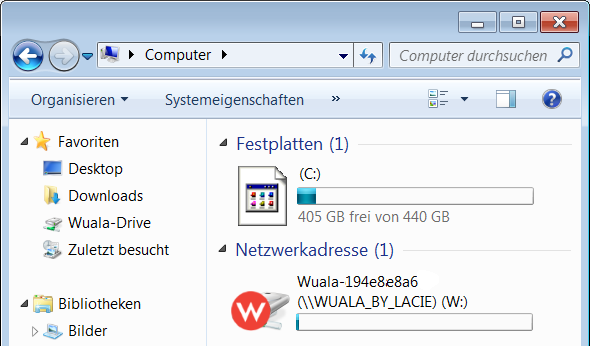
\includegraphics[scale=0.45]{../screenshots/wuala-drive.png}
\caption{Wuala-Laufwerk im Windows Explorer}
\label{abb:wualadrive}
\end{center}
\end{figure}